%==============================================================================
% Sjabloon onderzoeksvoorstel bachproef
%==============================================================================
% Gebaseerd op document class `hogent-article'
% zie <https://github.com/HoGentTIN/latex-hogent-article>

% Voor een voorstel in het Engels: voeg de documentclass-optie [english] toe.
% Let op: kan enkel na toestemming van de bachelorproefcoördinator!
\documentclass{hogent-article}
\usepackage{lipsum} % Voor vultekst
\usepackage{tabularx} % Voor tabellen met vaste breedte
\usepackage{pifont}
\usepackage{rotating}
\usepackage{pdflscape}

\usepackage[capposition=top]{floatrow}

% Invoegen bibliografiebestand
\addbibresource{voorstel.bib}

% Informatie over de opleiding, het vak en soort opdracht
\studyprogramme{Professionele bachelor toegepaste informatica}
\course{Bachelorproef}
\assignmenttype{Onderzoeksvoorstel}
% Voor een voorstel in het Engels, haal de volgende 3 regels uit commentaar
% \studyprogramme{Bachelor of applied information technology}
% \course{Bachelor thesis}
% \assignmenttype{Research proposal}

\academicyear{2024-2025}

% TODO: Werktitel
\title{Low-code softwareontwikkeling: Een vergelijkende studie van low-code platformen voor de digitalisatie van KMO’s}

% TODO: Studentnaam en emailadres invullen
\author{Glenn Vereecken}
\email{glenn.vereecken@student.hogent.be}

% TODO: Geef de co-promotor op
\supervisor[Co-promotor]{B. Goossens (Green Bananas, \href{mailto:ben@greenbananas.be}{ben@greenbananas.be})}

% Binnen welke specialisatierichting uit 3TI situeert dit onderzoek zich?
% Kies uit deze lijst:
%
% - Mobile \& Enterprise development
% - AI \& Data Engineering
% - Functional \& Business Analysis
% - System \& Network Administrator
% - Mainframe Expert
% - Als het onderzoek niet past binnen een van deze domeinen specifieer je deze
%   zelf
%
\specialisation{Mobile \& Enterprise development}
\keywords{Low-code, webapplicatie, software ontwikkeling, digitalisatie, KMO's}

\begin{document}

\begin{abstract}
  In een snel evoluerende technologische maatschappij groeit de behoefte aan digitalisering dagelijks. Bedrijven kunnen steeds meer waarde vinden in een digitale voetafdruk. Sinds de coronapandemie zijn jongere generaties vertrouwd geraakt met online winkelen, waardoor deelname aan de digitale markt essentieel is geworden. Voor veel bedrijven, vooral KMO’s, verloopt dit echter niet soepel. Velen hebben geen of een zwakke online aanwezigheid en beschikken niet over IT-personeel of de middelen om dit aan te nemen. Dit onderzoeksvoorstel onderzoekt welk low-code platform het meest geschikt is voor kleine tot middelgrote bussinesses om zelf een website te ontwikkelen. De volgende methode wordt gehanteerd: uit een breed aanbod aan low-code platformen wordt een selectie gemaakt op basis van vooraf gedefinieerde vereisten. Voor elk geselecteerd platform wordt een website gemaakt om het platform te testen en evalueren. Verwacht wordt dat de resultaten van dit onderzoek bedrijven zullen helpen bij het kiezen van het meest geschikte low-code platform voor de digitalisering van KMO’s.\end{abstract}

\tableofcontents

% De hoofdtekst van het voorstel zit in een apart bestand, zodat het makkelijk
% kan opgenomen worden in de bijlagen van de bachelorproef zelf.
%---------- Inleiding ---------------------------------------------------------

% TODO: Is dit voorstel gebaseerd op een paper van Research Methods die je
% vorig jaar hebt ingediend? Heb je daarbij eventueel samengewerkt met een
% andere student?
% Zo ja, haal dan de tekst hieronder uit commentaar en pas aan.

\paragraph{Opmerking}

 Dit voorstel is gebaseerd op het onderzoeksvoorstel dat werd geschreven in het
 kader van het vak Research Methods dat ik vorig academiejaar heb
 uitgewerkt met medesturent Duym Aron als mede-auteur.
 
\section{Inleiding}%
\label{sec:inleiding}

\subsection{Context}
\label{sec:Context}

De digitalisering van de maatschappij is de afgelopen jaren sterk toegenomen, waardoor bedrijven steeds vaker een digitale voetafdruk nodig hebben \autocite{schwab2016fourth}. \textcite{almeida2020challenges} stellen dat er sinds de coronapandemie een duidelijke drang naar of zelfs eis tot digitalisering is ontstaan. Bij deze digitalisering doen zich echter twee problemen voor: een gebrek aan IT-kennis binnen het bedrijfsleven \autocite{kutnjak2021covid} en een tekort aan ICT-professionals of de mogelijkheid om deze aan te nemen \autocite{VDAB2024}. 

\vspace{\baselineskip}

De covid-pandemie dwong bedrijven zich snel op de digitale markt te positioneren vanwege de plotselinge overgang naar lockdown. Jongere generaties raakten tijdens de pandemie vertrouwd met webshops \autocite{almeida2020challenges}, waardoor het voor achterblijvende bedrijven noodzakelijk werd om snel en eenvoudig te digitaliseren. Volgens \textcite{findikoglu2011small} verkiezen kleine tot middelgrote bedrijven het werken met locale service-providers, aangezien het makkelijker is om een vertrouwensband te vormen op lokale basis. Low-code kan een mogelijke oplossing bieden voor de efficiënte ontwikkeling van websites en applicaties zodat kleinere, locale IT-bedrijven meer contracten kunnen aannemen. 

\vspace{\baselineskip}

Volgens \textcite{bock2021low} is Low-code (LC) een relatief nieuwe programmeermethode die \\sinds het einde van de jaren 2010 snel aan populariteit wint. hij vermeldt verder dat low-code platforms (LCP’s) een grafische gebruikersinterface (GUI) bieden waarmee ontwikkelaars applicaties kunnen bouwen met minimale hoeveelheden code. Als laatste merkt hij op dat het aantal bedrijven dat LCP's aanbiedt elk jaar groeit en zowel kleine bedrijven als tech-giganten zoals IBM, Microsoft en Oracle omvat.

\subsection{Probleemstelling}
\label{sec:Probleemstelling}

Een groot probleem bij kleine tot middelgrote bedrijven is het ontbreken van een adequate digitale voetafdruk. Vaak zijn deze bedrijven niet in staat om zelf een website te maken of gebruiken zij een sterk verouderde site. Een moderne website is belangrijk doordat jongere generaties sinds de coronapandemie meer en meer vertrouwd zijn geraakt met online shopping. Dit onderzoeksvoorstel tracht deze bedrijven te ondersteunen door lokale IT-bedrijven te helpen om efficiënter webapplicaties te kunnen maken met behulp van low-code.

\subsection{Onderzoeksvraag}
\label{sec:Onderzoeksvraag}

Gezien de sterk evoluerende trend naar digitalisering, is het interessant om te onderzoeken hoe kleine tot middelgrote bedrijven zich kunnen digitaliseren. De focus ligt hierbij op het ontwikkelen van een persoonlijke website met mogelijke integratie van een webshop. De onderzoeksvraag luidt als volgt: 
 
\vspace{\baselineskip}

\begin{itemize}
  \item Welk low-code ontwikkelingsplatform voldoet het best aan de eisen voor de ontwikkeling van een moderne website voor kleine tot middelgrote bedrijven?
\end{itemize}

\subsubsection{Subvragen}
\label{sec:Subvragen}
\begin{itemize}
  \item Welk low-code ontwikkelingsplatform is de meest betaalbare optie voor kleine bedrijven?
  \item Welk low-code ontwikkelingsplatform biedt de meeste functionaliteiten en customisatie aan de gebruiker?
  \item Welk low-code ontwikkelingsplatform is het gemakkelijkst te gebruiken voor \\IT-personeel?
\end{itemize}
 
\subsection{Onderzoeksdoelstelling}
\label{sec:Onderzoeksdoel}

Dit onderzoek richt zich op het ondersteunen van kleine IT-bedrijven met een beperkte personeelscapaciteit door hun een mogelijke oplossing te bieden waarmee zij sneller kunnen ontwikkelen. De focus ligt op het ontwikkelen van een moderne website voor KMO’s, een essentiële benodigdheid in de moderne wereld. Het doel van het onderzoek is te evalueren welke low-code ontwikkelingsplatformen het meest geschikt zijn voor deze IT-bedrijven om een website te bouwen.

\subsection{Structuur van het onderzoek}
\label{sec:Structuur van het onderzoek}

\begin{itemize}
  \item \hyperref[sec:literatuurstudie]{Hoofdstuk 2} bespreekt de literatuurstudie en de stand van zaken rondom low-code. Dit onderdeel verduidelijkt wat low-code en low-code platformen precies zijn. Verder wordt er gekeken naar welke componenten zorgen voor een goede en moderne website. Tenslotte wordt er nog gekeken naar voorgaand onderzoek en onderzoek in verband met de leerbaarheid van low-code platformen.
  \item \hyperref[sec:methodologie]{Hoofdstuk 3} geeft uitleg over de methodologie die gebruikt zal worden tijdens dit onderzoek. Eerst wordt de requirements-analyse besproken. Vervolgens worden de longlist en de shortlist besproken. Daarna wordt de proof of concept van dit onderzoek besproken. Tenslotte wordt er nog gesproken over de verwerking van de data die uit de proof of concept en de conclusie die daaruit voortvloeien.
  \item \hyperref[sec:Verwachte resultaten]{Hoofdstuk 4} bespreekt de verwachte resultaten die verzameld zijn op basis van de literatuurstudie en de methodologie. Dit schept een duidelijk beeld van de informatie die met dit onderzoek is verkregen. 
  \item \hyperref[sec:discussie-conclusie]{Hoofdstuk 5} bespreekt de verwachte conclusies uit het onderzoek. In deze conclusie wordt een antwoord gegeven op de onderzoeksvraag en de bijbehorende subvragen.
\end{itemize}

%---------- Stand van zaken ---------------------------------------------------

\section{Literatuurstudie}%
\label{sec:literatuurstudie}

In de eerste hoofdstukken van deze literatuurstudie worden belangrijke termen gedefinieerd. Vervolgens worden de verschillen tussen low-code en no-code platforms verkend, waarbij wordt besproken hoe beide werken en voor welk publiek ze bedoeld zijn. Daarna komt de opzet van een moderne website aan bod, met een focus op welke elementen bijdragen aan het succes ervan. Ook wordt eerder onderzoek naar low-code onderzocht om een beter inzicht te krijgen in de voordelen en beperkingen die in eerdere studies zijn vastgesteld.

\subsection{Definities}
\label{sec:Definities}

\textbf{Low-code}: low-code is een meer visuele manier van softwareontwikkeling waarbij ontwikkelaars gebruik kunnen maken van een grafische interface die reeds bestaande codefragmenten gebruikt om te programmeren. In tegenstelling tot pure code moet de programmeur veel minder code zelf schrijven. Bij low-code wordt er wel nog vanuit gegaan dat de programmeur zelf nog onderdelen van software codeert dat niet kan gedaan worden aan de hand van het low-code platform. \autocite{Spain2022}

\vspace{\baselineskip}

\textbf{No-code}: no-code is een manier van softwareontwikkeling waarbij de gebruiker zelf geen code hoeft te schrijven. Het interessante aan no-code platformen is dat er weinig tot geen programmeerkennis voor nodig is om deze te kunnen gebruiken. Met behulp van het no-code platform kan de gebruiker zelf zijn volledige applicatie ontwikkelen in een grafische interface zonder te hoeven weten hoe de achterliggende processen werken. \autocite{Kirvan2024}

\vspace{\baselineskip}

\textbf{Citizen developer}: Een citizen developer is een medewerker binnen een organisatie zonder formele opleiding of achtergrond in softwareontwikkeling, die zich bezighoudt met het ontwikkelen en onderhouden van softwareapplicaties. Dit gebeurt meestal via een low-code of no-code ontwikkelingsplatform, waarmee deze ontwikkelaar op eenvoudige en gebruiksvriendelijke manier aan softwareontwikkeling kan doen zonder daarvoor kennis nodig te hebben van het programmeren. Vaak zijn citizen developers afkomstig uit de zakelijke kant van het bedrijf. \autocite{Kirvan2023}

\subsection{Low-code vs No-code}
\label{sec:Low-code vs No-code}

Volgens \textcite{Oluwaseyi2024} is het grootste verschil tussen deze twee programmeerstijlen voornamelijk de doelgroep. Zowel low-code als no-code zijn beide manieren om software te ontwikkelen op basis van een GUI met vooraf gedefinieerde componenten. Hij beweert dat bij low-code het platform hoofdzakelijk gericht is op programmeurs die ervaring hebben met programmeren en begrijpen wat er achterliggend allemaal gebeurt bij een applicatie. Vervolgens zegt \textcite{Oluwaseyi2024} dat bij no-code het product meer gericht is op zogenaamde “citizen developers” of mensen uit de business die geen voorafgaande kennis hebben van programmeren. Hierbij wordt het volledige ontwikkelingsproces zo veel mogelijk vereenvoudigd tot simpele componenten waarvan de code niet kan worden gewijzigd. Hij beweert ook dat low-code daarentegen de gebruiker meer de mogelijkheid zal geven om componenten aan te passen of te wijzigen. Met deze ondervindingen duidt \textcite{Oluwaseyi2024} een zeker verschil aan in de flexibiliteit en manier van werken tussen beide werkwijzen.

\vspace{\baselineskip}

Volgens \textcite{ICE2022} is er tenslotte ook nog een verschil in doel. \textcite{ICE2022} beweert dat het hoofddoel van low-code is om vaste ontwikkelingsprocessen te versnellen door de programmeur te voorzien van flexibele codeblokken, zodat er niet te lang stilgestaan moet worden bij deze onderdelen van het ontwikkelingsproces. \textcite{ICE2022} zegt ook dat bij no-code het vooral de bedoeling is om mensen met weinig tot geen programmeerkennis de mogelijkheid te geven om hun eigen applicaties te bouwen op een gebruiksvriendelijke manier.

\subsection{Layout van een moderne website}
\label{sec:Layout van een moderne website}

Hoewel webdesign niet de kern van dit onderzoeksvoorstel is, is het van belang kort te bespreken welke factoren een website succesvol maken. User engagement, user satisfaction en gebruiksvriendelijkheid zijn cruciale elementen bij het ontwikkelen van een website. User satisfaction en gebruiksvriendelijkheid kunnen samengevoegd worden om aan te geven dat het vooral gaat om het gebruiksgemak. Onderzoek van onder andere \textcite{vila2021indicators}, \textcite{saoula2023building} en \textcite{flavian2009web} ondersteunt dit.

\vspace{\baselineskip}

User engagement verwijst naar het daadwerkelijk gebruiken van een website door gebruikers, wat bij een webshop ook betrekking heeft op het stimuleren van verkoop. \textcite{garett2016literature} identificeren navigeerbaarheid, visualisatie en lay-out als de belangrijkste elementen van user engagement.

\vspace{\baselineskip}

Navigeerbaarheid betreft de mogelijkheid voor de gebruiker om zich binnen een website te navigeren. Volgens onderzoek van \textcite{vila2021indicators} begint 70\% van de gebruikers met zoeken zonder precies te weten wat en hoe ze willen zoeken. Daarom is de bruikbaarheid en herkenbaarheid van navigatie componenten essentieel om frustratie bij gebruikers te voorkomen.

\vspace{\baselineskip}

Visualisatie slaat op het visueel en ordelijk representeren van data en bijvoorbeeld ook producten in een webshop. Het principe van visual marketing stelt dat klanten eerder geneigd zijn iets te kopen als ze kunnen zien hoe een product eruitziet. \textcite{saoula2023building} tonen aan dat een visueel en ordelijk gepresenteerde website het vertrouwen van gebruikers vergroot, wat hen stimuleert om terug te keren.

\vspace{\baselineskip}

Lay-out is belangrijk in twee opzichten: kleurgebruik en de presentatie van verschillende elementen van een website. Volgens \textcite{beaird2020principles} is het belangrijkste aan een lay-out dat een website voelt als een geheel. Verder vindt hij dat een goede mix aan content en zogenaamde "whitespace" essentieel is bij het ontwerpen van een goede lay-out.

\vspace{\baselineskip}

Responsiviteit voor verschillende apparaten is eveneens cruciaal. \textcite{wagner2020online} constateerden dat in 2017 wereldwijd 49\% van de online shoppers gebruikmaakte van hun pc, terwijl 51\% gebruikmaakte van mobiele apparaten zoals smartphones en tablets. Hedendaags is dit percentage voor de mobiele markt gestegen tot meer dan 60\% van de totale online shoppers \autocite{Seitz2024}.

\subsection{Voorgaand onderzoek}
\label{sec:Voorgaand onderzoek}

In de laatste jaren is het gebruik van low-code en het onderzoek hiernaar sterk in opmars. Steeds meer applicaties worden ontwikkeld met behulp van low-code. \textcite{GartnerResearch2019} voorspelde in 2019 dat tegen 2024 meer dan 65\% van alle ontwikkelingsprojecten gebruik zullen maken van \\low-code voor de ontwikkeling van hun applicaties. Een onderzoek van \textcite{VanMullem2022} onderzoekt of traditioneel programmeren volledig kan worden vervangen door low-code. Hij concludeert dat ongeveer 95\% van processen kunnen worden gemodelleerd met behulp van een LCP, de overige 5\% bevat taken die te complex waren voor low-code platformen.

\subsection{De bruikbaarheid van low-code}
\label{sec:De bruikbaarheid van low-code}

Volgens het boek van \textcite{kenneweg2021building} kan elke geïnteresseerde persoon applicaties maken met behulp van een low-code platform. Voorafgaande kennis in softwareontwikkeling is niet noodzakelijk om met low-code applicaties te werken volgens hen, hoewel het wel een pluspunt kan zijn om het leer- en werkproces te vereenvoudigen.

\vspace{\baselineskip}

\textcite{rokis2022challenges} stellen dat low-code technologieën veel uitdagingen met zich meebrengen. Volgens hen zouden deze platforms een gebrek hebben aan methoden en benaderingen ter ondersteuning. Dit probleem kan volgens hen worden verminderd door de documentatie en leermiddelen van low-code platforms te verbeteren. \textcite{bernsteiner2022citizen} merken op dat de huidige documentatie vaak geschreven is voor professionele developers, wat het aanleren van deze software makkelijker maakt voor actieve ontwikkelaars.

%---------- Methodologie ------------------------------------------------------
\section{Methodologie}%
\label{sec:methodologie}

\begin{figure*}[p]
  \centering
  \scalebox{1.10} {%
  \rotatebox{90}{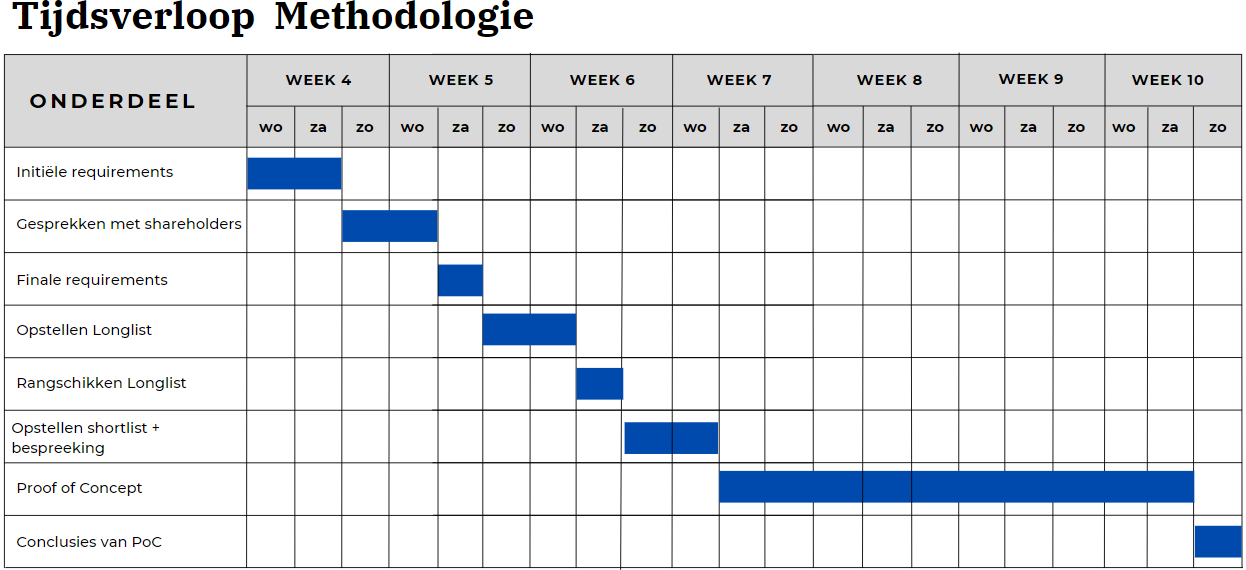
\includegraphics[width=\pdfpagewidth]{../graphics/Timetable4.png}}
  }
  \label{fig:your-figure-label}
  \caption[Tijdsverloop methodologie:]{Deze tabel toont het verwachte tijdsverloop van de methodologie en de geschatte duur van elke fase.}
  \floatfoot{*Er wordt aangenomen dat er op woensdag een volledige dag gewerkt kan worden aan de methodologie, deze dag kan verschillen.}
\end{figure*}

\subsection{Requirements analyse}
\label{sec:Requirements analyse}

De eerste stap in het effectieve onderzoek is het opstellen van een requirements-analyse, waarbij eisen voor low-code applicaties worden opgelijst en gerangschikt volgens de MoSCoW-metho\-de. Voor een concrete en volledige lijst van eisen worden twee bronnen geraadpleegd. Ten eerste wordt voorgaande literatuurstudie gebruikt om bepaalde noodzakelijke eisen te identificeren. Deze eerste stap kan twee dagen duren. Daarna worden gesprekken gevoerd met stakeholders, zoals de school en de promotors, om de bevindingen uit stap één te beoordelen en te toetsen. Eventuele aanvullingen of nieuwe eisen kunnen worden toegevoegd. Voor deze gesprekken wordt één dag per groep stakeholders gerekend. Vervolgens wordt nog één dag ingepland voor het finaliseren van de requirements-analyse.

\subsection{Longlist}
\label{sec:Longlist}

Na het samenstellen van een requirementsanalyse is het belangrijk een longlist van low-code platformen samen te stellen op basis van deze analyse en de informatie uit de literatuurstudie. Voor het onderzoeken van low-code platformen en het samenstellen van de longlist is een tijdsduur van twee dagen voorzien.
Deze lijst met low-code platformen wordt gerangschikt aan de hand van de volledige lijst van requirements. Deze stap kan één dag in beslag nemen, afhankelijk van de huidige opgelijste requirements. De rangschikking wordt weergegeven in een tabel, waarbij de best scorende platformen zich bovenaan bevinden.

\subsection{Shortlist}
\label{sec:Shortlist}

Bij het opstellen van de shortlist wordt gekeken naar de drie platformen die het best voldoen aan de vereisten uit de requirementsanalyse. Deze drie zullen elk individueel uitgebreid worden besproken. Hierbij komt aan bod wat het platform exact kan, waarvoor het meestal wordt gebruikt en welke programmeertaal achterliggend wordt gebruikt. Daarnaast worden de prijsstructuren van de platformen geanalyseerd om te bepalen welke het meest geschikt is voor kleine tot middelgrote ondernemingen.

\subsection{Proof of concept}
\label{sec:Proof of concept}

\subsubsection{Uitleg}
\label{sec:Uitleg}

Voor de proof of concept van dit onderzoek zal getest worden welk low-code platform het best voldoet aan de vooropgestelde eisen uit de requirementsanalyse. Hiervoor wordt met elk low-code platform uit de shortlist een moderne website gemaakt op basis van een meegegeven ontwerp. Dit ontwerp wordt samen opgesteld met onze stakeholders en besproken in een later onderdeel.

\subsubsection{Beschrijving website}
\label{sec:Beschrijving website}

De te ontwikkelen websites zijn moderne websites met een startpagina, een over-ons pagina, een login functionaliteit en een eenvoudige webshop tot aan het punt van betaling. Deze websites maken gebruik van een SQLite-database voor het opslaan van artikelen en gegevens, indien het platform geen eigen database voorziet. Qua styling wordt er vastgehouden aan moderne design principes, bepaald door een vooraf opgesteld ontwerp. Het belangrijkste aspect van deze opdracht is het creëren van een functionele website met de gevraagde pagina’s.

\subsubsection{Manier van onderzoek}
\label{sec:Manier van onderzoek}

Ten eerste wordt één dag per low-code platform gereserveerd om kennis te maken met het platform en het gebruik ervan te leren. Hierbij wordt ook de gebruiksvriendelijkheid en de aanwezige features van het platform beoordeeld. Vervolgens wordt met elk platform de vooraf beschreven website gemaakt.

\vspace{\baselineskip}

Tijdens de ontwikkeling van de site logt de ontwikkelaar zijn tijd voor beide applicaties. De gewerkte uren worden bijgehouden en meegenomen in de beoordeling van de gebruiksvriendelijkheid van het platform.

\subsection{Verwerking proof of concept data}
\label{sec:Verwerking proof of concept data}

Na het leren van de low-code platformen en het ontwikkelen van de websites worden de eindresultaten geëvalueerd. Eerst worden de eindproducten vergeleken met het originele ontwerp en krijgen zij een score op basis van design, functionaliteiten en de tijdsduur van het hele ontwikkelingsproces volgens de vereisten uit de requirementsanalyse. Vervolgens wordt het analyseproces beoordeeld op hoe vlot het leerproces was om het low-code platform te leren gebruiken. Indien een website na drie dagen nog niet volledig afgewerkt is, wordt dit opgenomen in de eindscore.

\subsection{Conclusie proof of concept}
\label{sec:Conclusie proof of concept}

Na het verwerken van de data en het evalueren van de criteria worden in de laatste fase conclusies getrokken over wat goed is gegaan en welke aspecten gebreken vertoonden. Vervolgens worden de low-code platformen gerangschikt op basis van de onderzoeksvraag en op basis van elke subvraag. 

%---------- Verwachte resultaten ----------------------------------------------
\section{Verwacht resultaat, conclusie}%
\label{sec:verwachte_resultaten}
Er wordt verwacht dat uit de conclusie van de proof of concept er per categorie één bepaald low-code platform als meest geschikt zal worden geïdentificeerd. Deze platforms zullen vervolgens worden besproken om te verklaren waarom zij het beste zijn voor hun respectieve subvraag. Bedrijven zullen zelf moeten bepalen welk platform het beste bij hen past. Per platform wordt een ranking gegeven van hoe goed ze presteren in de verschillende categorieën, om te bepalen welk platform het meest voldoet aan de eisen die in dit onderzoek zijn opgesteld.

\section{Discussie, verwachte conclusie}
\label{sec:discussie-conclusie}

De resultaten van dit onderzoek zullen kleine IT-bedrijven ondersteunen bij het selecteren van een geschikt low-code platform voor de ontwikkeling van websites voor KMO's. Hierdoor kunnen zij hopelijk meer contracten opnemen en hun winstmarges vergroten. Verder wordt aanbevolen om in de toekomst meer onderzoek te verrichten om nieuwe of verbeterde low-code platforms te evalueren en te vergelijken zodat bedrijven op lange termijn kunnen blijven profiteren van de nieuwste technologische ontwikkeling. 

\printbibliography[heading=bibintoc]

\end{document}